\chapter{Experimental Methodology}
This chapter will introduce the reader to the methodology used to experiment our work. This includes the data sets we have generated and their difference in distributions, which have helped us find key differences in the performances of our implementations. Later in this chapter we present the experimental environment, which includes the hardware and software we have used and finally we conclude with an evaluation of the experiments we have created and the reasons why.

\label{chapter:experimentalmethodology}
\section{Data generation}
Until this point, all implementations have been tested and validated on examples from the book (\textit{book.in}). Doing this helps determine the correctness of the implementations and gives some hints about the running times of each version, however, book.in is too small to draw any meaningful conclusions from it. To challenge the implementations we have created a simple dataset generator, which works with several different distributions. This chapter will introduce the reader to the dataset generator and the sets that were generated to put the implementations to test and help discover performance differences.   

\subsection{Generator Overview}
The generator is implemented in C\texttt{++} and takes 3 arguments as input - total number of options in the set, a skewness parameter and the data distribution type to be generated. The inputted number of options is used as a max limit when generating options. We have generated six essential datasets with $2^{16}=65536$ options, which is double the total number of available threads on the GPU that was used for this thesis\footnote{Hardware will be described later in section~\ref{section:experimental:enviornment}} (32768). Additionally, we have created variations for each essential data distribution with $1000$, $10000$ and $30000$ options in each (that is $6*3=18$ more files), which could be useful to test performance differences when files have different number of options. 

The skewness parameter represents the amount (in percent) of options that will be skewed (have significantly different height and/or width than the rest of the options). This parameter is applied only for the skewed distributions, which will be described later in this chapter. Lastly, the data distribution type is used to specify the dataset which will be generated. The generator currently works with 6 different types, which will be described next in this section. Plots and statistics to show the data distributions are available in Appendix \ref{appendix:data}. Note that all data distribution plots consist of a scatter plot where each dot represents an option, and histogram plots next to their corresponding axis, indicating on the data distribution. We have additionally included statistics for both the widths and the heights of different options in the file.

\subsection{Uniform}
The uniform data distribution consists of the same option replicated multiple times. Each entry in this set has the same height and the same width as the others. All widths in the newly generated set are equal to 47 and all heights to 109. As this set is uniformly distributed, all other statistics such as variance, std, skewness are 0 for both widths and heights. The data distribution and statistics about it are shown on fig.~\ref{fig:experimentmethodology:uniform}, where it can be seen that a dot is formed in the center of the plot. While pricing the same option this many times is not practically/financially useful, there is a possibility that many real-life inputs will have a uniform distribution, where both their widths and heights will have close values. In such a case, the dots on the plot will be separated, but will still remain close to the center. This suggests that in these distributions, pricing individual options will also take similar times. In our generated set, each option should be priced in exactly the same amount of time. Furthermore, since there is no difference in the heights and the widths, it is not expected that pricing this data distribution in parallel will benefit from any sorting or padding, which should be an interesting experiment. 
\begin{figure}[H]
	\centering
	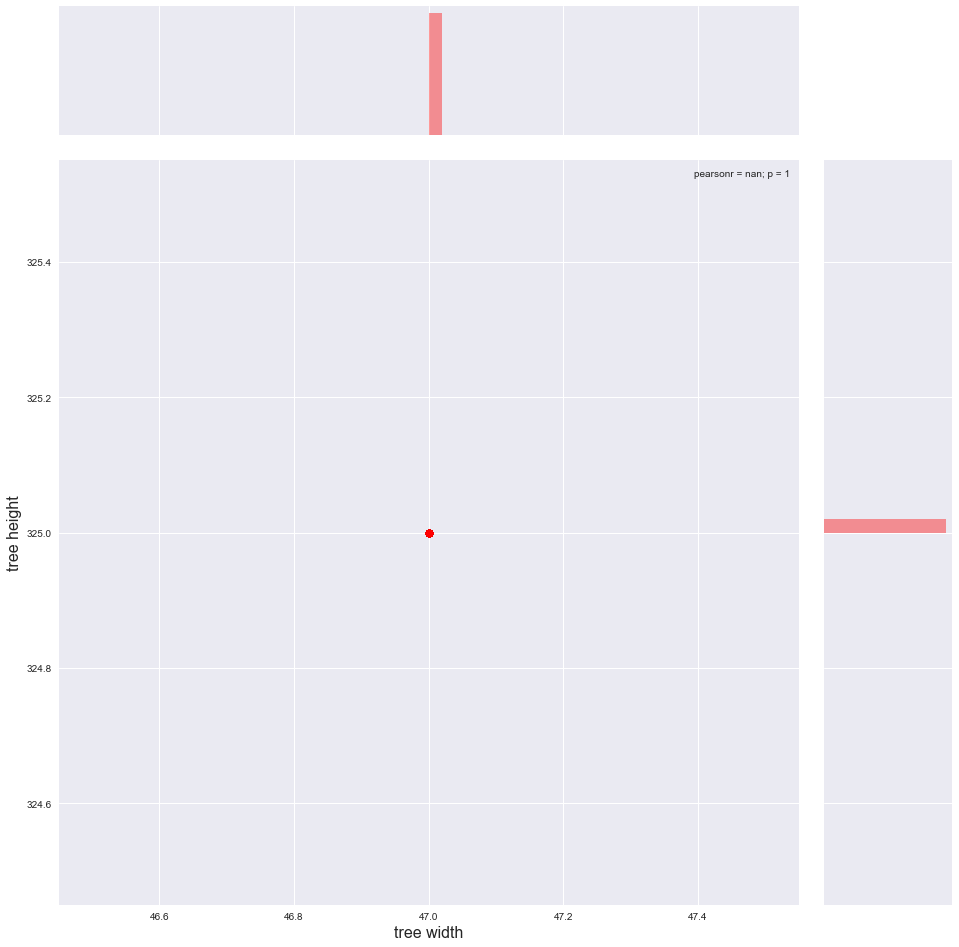
\includegraphics[width=0.7\textwidth]{img/0_UNIFORM_plot.png}
	\caption{Illustration of the uniformly distributed generated file}
	\label{fig:experimentmethodology:uniform}
\end{figure}

\subsection{Random}
The random data distribution (see fig. \ref{fig:experimentmethodology:random}) consists of options with both uniformly distributed random widths and uniformly distributed random heights. This dataset is interesting, as it presents a wide variety of option sizes. Both padding and sorting can benefit the processing of such a data distribution, hence it can help answer questions concerned with the various optimization techniques that can possibly improve the performance of the algorithm.

\begin{figure}[H]
	\centering
	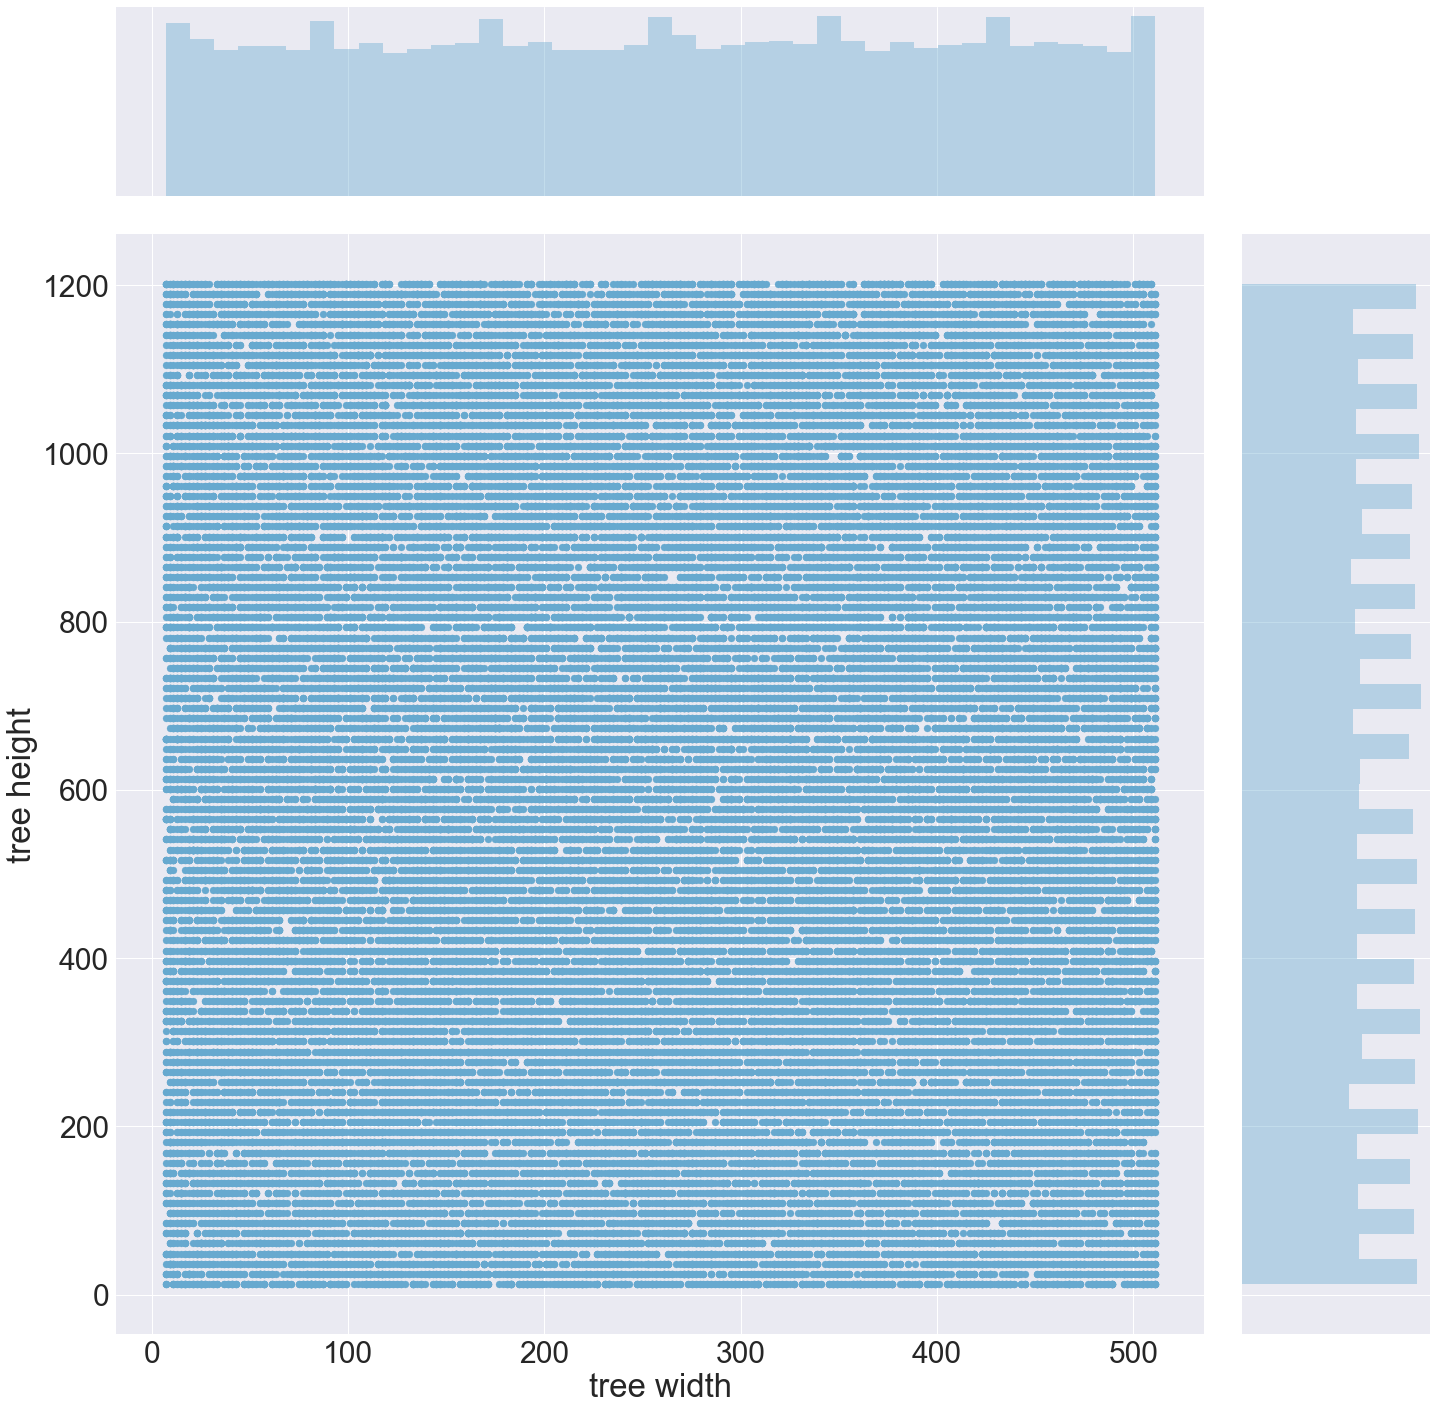
\includegraphics[width=0.7\textwidth]{img/1_RAND_plot.png}
	\caption{Illustration of the randomly distributed generated file}
	\label{fig:experimentmethodology:random}
\end{figure}

\subsection{Random with Constant Height/Width}
The following two data distributions (see Appendix \ref{appendix:data} for plots and details) have similar structures as the random one described above, however, one of their parameters is being held in place (kept constant). In the case of constant height, the width is uniformly randomly distributed, while the height remains the same throughout all options. The other case is vice verse, where the width remains the same, while the height is randomly distributed. It will be interesting to experiment whether having a constant width or height benefits the performance of any implementation. It should also be interesting to see if sorting and padding can benefit the performance. 

\subsection{Skewed}
This data distribution introduces data skewness, where a small percent of all options is significantly different than the rest. As it can be seen on fig. \ref{fig:experimentmethodology:skewed}, the majority of the data has widths up to approx. 100 and heights up to approx. 400. Several options with much larger heights and widths stand out with a larger range for both widths and heights. This data distribution can also often occur in real life situations, where several data entries significantly deviate from the rest. This introduces problems with memory padding in some of the implementations, but can benefit from sorting both along the height and along the width. It will be interesting to experiment with the behaviour of \textit{CUDA-multi} on similar datasets where the majority of options have small widths, hence allowing to pack and process more options in parallel. 

\begin{figure}[H]
	\centering
	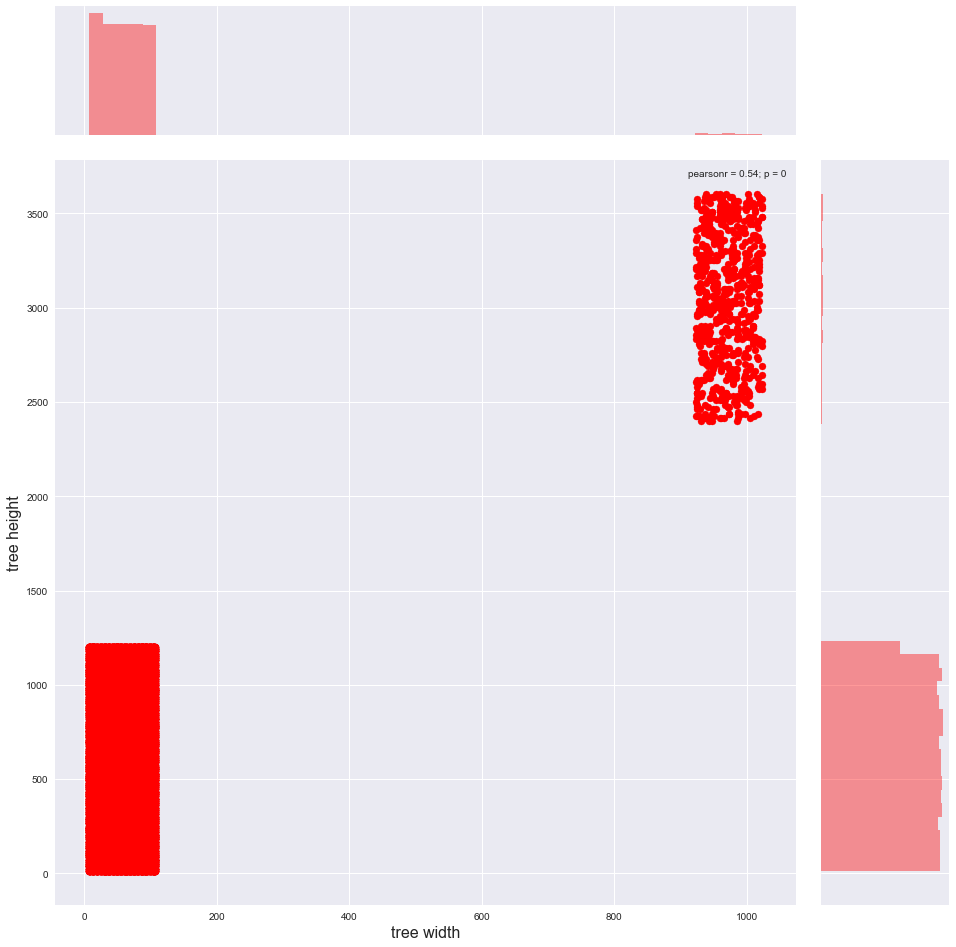
\includegraphics[width=0.7\textwidth]{img/4_SKEWED_plot.png}
	\caption{Illustration of the skewed generated file}
	\label{fig:experimentmethodology:skewed}
\end{figure}

\subsection{Skewed with Constant Height/Width}
The last two data distributions (see Appendix \ref{appendix:data} for plots and details) introduce similar concepts as the skewed dataset. Similarly, the majority of the data has a relatively small uniform random distribution on both axes. The difference comes in the skewed part, where either the height or the width are constant, with a much larger values than the rest of the set. Тhe free parameter (the one that is not held constant) in these cases has the same distribution as the rest of the options. These two sets can show interesting information about the dominance of either widths or heights in a dataset, and help determine whether any of the implementations perform better on widths or on heights. It should also be interesting to observe the runtime when sorting and padding are used on each of the different axes. 

\section{Experimental Environment}\label{section:experimental:enviornment}
\paragraph{Hardware}
In order to test our code, we have used the GPU cluster at DIKU\footnote{Find more information on \url{https://di.ku.dk/it/documentation/gpu/}}. It is composed of 5 servers with multicore CPUs and 2 GPUs per machine. We have only used four of the machines (GPU01-04) each with 2 x \textit{nVidia GeForce GTX 780 GPUs}. The complete hardware specification for each of the 4 GPUs is described below:
\begin{itemize}
\item \textbf{Case}: 1x Supermicro SYS-7047GR-TPRF, 4U/Tower barebone LGA2011, 2x1620W PSU, 8x3.5" htswp trays

\item \textbf{CPU}: 2x Intel Xeon E5-2650v2, 8-core CPU, 2.6GHz, 20MB cache, 8GT/s QPI

\item \textbf{RAM}: 8x Samsung 16GB DDR3(128GB total) 1866MHz Reg. ECC server module

\item \textbf{GPU}: 2x nVidia GeForce GTX 780 Ti, 3072MB, 384 bit GDDR5, PCI-E 3.0 16x, 15 streaming multiprocessors with 2880 CUDA cores (single precision) and 960 CUDA cores (double precision) and compute capability 3.5

\item \textbf{SSD}: 1xIntel S3500 serie 240GB SATA

\item \textbf{HDD}: 1x	Seagate Constellation ES.3 4TB 7200RPM SATA 6Gb/s 128MB cache 3,5"
\end{itemize}

The GTX 700 series were first released in 2013 and GPU technology has noticeably improved since. Despite that, both CUDA and Futhark provide portability, allowing to easily switch hardware, or scale the solution, allowing to run the code on even more modern hardware, without the need to re-write it.

\paragraph{Software}
We also turn to software as another aspect of portability. Even though CUDA and Futhark allow code to be run on many different architectures and operating systems, it is often a good idea to align compiler versions on different systems. All experiments described in chapter \ref{chapter:experimentalresults} have been run on \textbf{Red Hat Enterprise Linux Server 7.5 (Maipo)} with a \textbf{Linux 3.10.0-862.6.3.el7.x86\_64} kernel. All CUDA programs have been compiled by \textbf{Cuda compilation tools, release 9.2, V9.2.148} using \textbf{C\texttt{++11}} and all Futhark programs by the \textbf{Futhark 0.6.0} compiler. Note that the use of older versions of both may result in compile errors, as we have used modern language features introduced in the newer releases. The same applies for newer compiler versions, since we cannot guarantee that neither Nvidia products, nor the Futhark language are going to be backward compatible.

\paragraph{Experiments}
With the large number of combinations between datasets, computation precision, implementations, optimizations and more, we have created a testing framework for our CUDA implementations. It runs one combination at a time and writes the measurements to a file. For each run we obtain the name of the file; the precision; number of registers; the implementation version; the block size; the sort option; kernel time in microseconds; total time in microseconds and the total allocated memory in bytes. Futhark implementations are tested using the built-in \textit{futhark-bench} tool.

\paragraph{Evaluation}
Throughout all experiments, we have tested for multiple performance factors:
\begin{itemize}
    \item Using both \textbf{float} and \textbf{double} precision. Although we do not expect that computing doubles will perform better than floats, it has been interesting to observe how the algorithms perform on different levels of precision.
    
    \item To determine the highest performing implementation, we evaluate the \textbf{runtimes} of all approaches. For simplicity, we align our CUDA findings with \textit{futhark-bench}'s measurement strategy - excluding input reading, device context initialization, copying of input and output to/from the device and writing the output. Pre-computations of the data, such as sorting and index computations/padding are still included in our results. It has been interesting to observe the speed-ups achieved when different variations of sorting were applied, when different types of padding were applied and when different block sizes were used\footnote{Note that \textit{CUDA-multi} is always expected to perform better with the largest block size available - namely 1024, hence we have tested different block-sizes only for \textit{CUDA-option}.}. All runtimes are in seconds, as we have found that measure to be best visually representative on the plots.
    
    \item Another important measurement we have considered was \textbf{memory}. We have created multiple versions both for \textit{CUDA-option} and \textit{CUDA-multi}, where memory was optimized, thus it has been interesting to observe the impacts of each version. Memory has been measured in megabytes (MB).
\end{itemize} 

\section*{Summary}
This chapter provided an overview of the methodology used in order to set up the experiment environment. This has included the datasets we have generated in order to put the implementations to a test, the hardware and software used to run them and a brief description of what exactly we have put to the test in order to measure performance. The following chapter will introduce the actual experiments and elaborate on the results we have obtained, in order to determine different performance characteristics and obtain an empirical validation for answering the thesis questions.